
% This is "bach-ref-2009.tex" Updated january 29th 2010.
% This file should be compiled with "sig-alternate-fixed.cls" January 2010.
% It is based on the ACM style "sig-alternate.cls"
% -------------------------------------------------------------------------
% This example file demonstrates the use of the 'sig-alternate-fixed.cls'
% V2.5 LaTeX2e document class file. It is for those submitting
% articles to the Twente Student Conference on IT. Both this file as the 
% document class file are based upon ACM documents.
%
% ----------------------------------------------------------------------------------------------------------------
% This .tex file (and associated .cls) produces:
%       1) The Permission Statement
%       2) The Conference (location) Info information
%       3) The Copyright Line TSConIT
%       4) NO page numbers
%       5) NO headers and/or footers
%
% Using 'sig-alternate.cls' you have control, however, from within
% the source .tex file, over both the CopyrightYear
% (defaulted to 200X) and the ACM Copyright Data
% (defaulted to X-XXXXX-XX-X/XX/XX).
% e.g.
% \CopyrightYear{2007} will cause 2007 to appear in the copyright line.
% \crdata{0-12345-67-8/90/12} will cause 0-12345-67-8/90/12 to appear in the copyright line.
%
% ---------------------------------------------------------------------------------------------------------------
% This .tex source is an example which *does* use
% the .bib file (from which the .bbl file % is produced).
% REMEMBER HOWEVER: After having produced the .bbl file,
% and prior to final submission, you *NEED* to 'insert'
% your .bbl file into your source .tex file so as to provide
% ONE 'self-contained' source file.
%

% refers to the cls file being used
\documentclass{sig-alternate-br}
\usepackage{float}
\usepackage{caption}
\usepackage{subcaption}
\usepackage{hyperref}
\restylefloat{figure}
\restylefloat{table}
\begin{document}

%
% --- Author Metadata here --- DO NOT REMOVE OR CHANGE 
%\conferenceinfo{13$^{th}$ Twente Student Conference on IT}{June 23$^{st}$, 2010, Enschede, The Netherlands.}
\CopyrightYear{2015} % Allows default copyright year (200X) to be over-ridden - IF NEED BE.
%\crdata{0-12345-67-8/90/01}  % Allows default copyright data (0-89791-88-6/97/05) to be over-ridden - IF NEED BE.
% --- End of Author Metadata ---

\title{micro data server using raspberry pi}
% In Bachelor Referaat at University of Twente the use of a subtitle is discouraged.
 \subtitle{Research Proposal}




\numberofauthors{1} 
\author{ 
% You can go ahead and credit any number of authors here,
% e.g. one 'row of three' or two rows (consisting of one row of three
% and a second row of one, two or three).
%
% The command \alignauthor (no curly braces needed) should
% precede each author name, affiliation/snail-mail address and
% e-mail address. Additionally, tag each line of
% affiliation/address with \affaddr, and tag the
% e-mail address with \email.
%
% 1st. author
\alignauthor P.j.e. Velthuis\\
       \affaddr{University of Twente}\\
       \affaddr{P.O. Box 217, 7500AE Enschede}\\
       \affaddr{The Netherlands}\\
       \email{p.j.e.velthuis@student.utwente.nl}
% 2nd. author
\alignauthor 2nd Author\\
       \affaddr{2nd author's affiliation}\\
       \affaddr{1st line of address}\\
       \affaddr{2nd line of address}\\
       \email{2nd author's email address}
% 3rd. author
\alignauthor 3rd Author\\
       \affaddr{3rd author's affiliation}\\
       \affaddr{1st line of address}\\
       \affaddr{2nd line of address}\\
       \email{3rd author's email address}
}

%\additionalauthors{Additional authors: John Smith (The
%Th{\o}rv{\"a}ld Group, email: {\texttt{jsmith@affiliation.org}})
%and Julius P.~Kumquat (The Kumquat Consortium, email:
%{\texttt{jpkumquat@consortium.net}}).}
%\date{30 July 1999}


\maketitle
\begin{abstract}
This document describes a draft research proposal in the
area of cloud computing services. The main research question
is: Is a cloud server consisting of Raspberry Pi efficient?
\end{abstract}

\keywords{Cloud computing, Raspberry Pi, ARM performance, micro data server}

\section{Motivation}
Today there are many cloud services. The amount of cloud computing services is increasing fast \cite{armbrust:2009}.  Despite the attention
from the research community, research and development of
Cloud Computing services is still in it's childhood\cite{tso:2013}. 
 In this research the Raspberry Pi cloud services will be investigated. A reason for this is that the density of servers has increased a lot in the past\cite{density}. There are new technologies such as for example the ARM processor. Many companies want to explore the possibilities of for example the Raspberry Pi and his ARM Processor. Some data centers even offer some cloud computing using the Raspberry Pi. A reason for this is the co-location and the low power usage of a Raspberry Pi\cite{hosting,Pcextreme}.  A Raspberry Pi has a power usage between the 3-5 Watt and a server has a power usage between the 75 and 150 watt \cite{Powerusage}. This could mean that it is better to use a Raspberry Pi for specific small tasks that do not demand a whole server. During this research I want to further investigate this power usage.  A Raspberry Pi can be the small data center for the future \cite{tso:2013}. The Raspberry is a rather cheap device for 35 euros. This makes it cheaper to do research in compared to a normal server. The current versions of the Raspberry Pi cannot perform the task of a large scale x86 server \cite{tso:2013}. Building a cloud like this can be a cost effective scale model\cite{tso:2013}. It's a Ideal testbed for testing distributed software. 




%\subsection{References and Citations}
%Footnotes should be Times New Roman 9-point, and justified to the 
%full width of the column.\footnote{A footnote in 9-point Times New Roman.}

%Use the "ACM Reference format" for references - that is, a numbered 
%list at the end of the article, ordered alphabetically and formatted 
%accordingly. See examples of some typical reference types, in the new 
%"ACM Reference format", at the end of this document. Within this 
%template, use the style named references for the text. Acceptable 
%abbreviations, for journal names, can be found here: 
%http://library.caltech.edu/reference/abbreviations/

%The references are also in 9 pt., but that section (see Section 7) is 
%ragged right. References should be published materials accessible to 
%the public. Internal technical reports may be cited only if they are 
%easily accessible (i.e. you can give the address to obtain the report 
%within your citation) and may be obtained by any reader. Proprietary
%information may not be cited. Private communications should be 
%acknowledged, not referenced  (e.g., "[Robertson, personal communication]")

%\subsection{Page Numbering, Headers and Footers}
%Do not include headers, footers or page numbers in your submission. 
%These will be added when the publications are assembled.

%\section{Figures / Captions}
%Place Tables/Figures/Images in text as close to the reference as possible 
%(See Figure \ref{fig:abc}).  It may extend across both columns. 

%\begin{figure}
%\centering 
%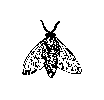
\epsfig{file=fly2.eps} 
%\caption{Insert caption to place below figure.}
%\label{fig:abc} %always place your label after your caption!
\ %end{figure}

%Captions should be Times New Roman 9-point bold.  They should be numbered (e.g., "Table 1" or "Figure 2"), please note that the word for Table and Figure are spelled out. Figure's captions should be centered beneath the image or picture, and Table captions should be centered above the table body.

%\section{Sections}
%The heading of a section should be in Times New Roman 12-point bold in all-capitals flush left with an additional 6-points of white space above the section head.  Sections and subsequent sub- sections should be numbered and flush left. For a section head and a subsection head together (such as Section 3 and subsection 3.1), use no additional space above the subsection head.

%\subsection{Subsections}
%The heading of subsections should be in Times New Roman 12-point bold with only the initial letters capitalized. (Note: For subsections and subsubsections, a word like the or a is not capitalized unless it is the first word of the header.)

%\subsubsection{Subsubsections}
%The heading for subsubsections should be in Times New Roman 11-point italic with initial letters capitalized and 6-points of white space above the subsubsection head.

%\section{Acknowledgments}
%Our thanks to ACM SIGCHI for allowing us to modify templates they had developed.

%\section{Introduction to Latex}
%Typically, the body of a paper is organized into a hierarchical
%structure, with numbered or unnumbered headings for sections,
%subsections, sub-subsections, and even smaller sections.  The
%command \texttt{{\char'134}section} that precedes this paragraph
%is part of such a hierarchy. \LaTeX\ handles the numbering and placement of these
%headings for you, when you use the appropriate heading commands
%around the titles of the headings.  If you want a sub-subsection
%or smaller part to be unnumbered in your output, simply append an
%asterisk to the command name.  Examples of both numbered and
%unnumbered headings will appear throughout the balance of this
%sample document.

%Because the entire article is contained in the \textbf{document}
%environment, you can indicate the start of a new paragraph with a
%blank line in your input file; that is why this sentence forms a
%separate paragraph.

%\subsection{Type Changes and {\subsecit Special} Characters}
%We have already seen several typeface changes in this sample.  You
%can indicate italicized words or phrases in your text with the
%command \texttt{{\char'134}textit}; emboldening with the command
%\texttt{{\char'134}textbf} and typewriter-style (for instance, for
%computer code) with \texttt{{\char'134}texttt}.  But remember, you
%do not have to indicate typestyle changes when such changes are
%part of the \textit{structural} elements of your article; for
%instance, the heading of this subsection will be in a sans

\section{Research questions}
The main research question
is: Is a cloud server consisting of Raspberry Pi efficient?

In order to come to a good answer we first need to build our own Raspberry Pi setup. There needs to be decided with which benchmark the performance will be measured. After we have measured the performance we can see   

\subsection{Citations}
Citations to articles \cite{bowman:reasoning, clark:pct,
braams:babel, herlihy:methodology}, conference proceedings
\cite{clark:pct} or books \cite{salas:calculus, Lamport:LaTeX}
listed in the Bibliography section of your article will occur
throughout the text of your article. You should use BibTeX to
automatically produce this bibliography; you simply need to insert
one of several citation commands with a key of the item cited in
the proper location in the \texttt{.tex} file
\cite{Lamport:LaTeX}. The key is a short reference you invent to
uniquely identify each work; in this sample document, the key is
the first author's surname and a word from the title.  This
identifying key is included with each item in the \texttt{.bib}
file for your article.

The details of the construction of the \texttt{.bib} file are
beyond the scope of this sample document, but more information can
be found in the \textit{Author's Guide}, and exhaustive details in
the \textit{\LaTeX\ User's Guide}\cite{Lamport:LaTeX}.

This article shows only the plainest form of the citation command,
using \texttt{{\char'134}cite}. This is what is stipulated in the
SIGS style specifications. No other citation format is endorsed or
supported.
\subsection{What is small scale cloud computing}
In this research I want to do some small scale cloud computing. The main motivation behind is is that it is ways to expensive to simulate large scale cloud computing. Another reason is the Co-location that can be used with small scale cloud computing. Because of this it could be better in executing small tasks. More motivation is that it does not use a lot of space and power. 
Eucalyptus https://www.eucalyptus.com/eucalyptus-cloud/get-started
Hazelcast

\subsection{What are the most promising cloud services}
In the PcExtreme article \cite{Pcextreme} there are running several services on a Raspberry Pi.
For example a webserver, a DNS server, a chat server, a mail server, a vpn server or a monitoring server. 
In this research I want to test some cloud services and programs to see if they are suitable for the Raspberry Pi. 
To investigate this I want to make a experimentation cloud with Raspberry Pi's to see if it will work as a cloud. 



\subsection{Is it reachable to build small personal Raspberry Pi clouds for services}
With this subquestion I want to find out if it is possible to let users have small Raspberry Pi servers such as now is happening at PcExtreme as an experiment. I also want to know what the performance of this small Raspberry Pi cloud is. 

\subsection{Is it possible to improve cloud programs using small scale Raspberry Pi's}


\section{Research Methods}
This research will investigate a cloud computer consisting of Raspberry Pi's. The research method for this would be the Design Science research method. this is a method to solve field problems. This research will make use of the design Science method proposed by Hevner\cite{hevner:2007}

\section{Research approach}
For the experiment we need a Raspberry Pi with a static Ip address and we need a sd card for the OS.  A Raspberry Pi can be used as a webserver or DNS server. For the experiment we need a Raspberry Pi B that can make use of the Ethernet.
In the setup video is explained how I can make such a cluster.
\url{https://www.youtube.com/watch?v=JtX9lVDsqzg}.
If I have made such I cluster I can start doing some tests on it. We will use applications also super computers will use such as Mpich. We will use Fortran to rank our raspberry pi server. 
I am for example curious about what the duration is between small seperated tasks and large tasks. 


Experiment making a VPN:
\url{http://readwrite.com/2014/04/10/raspberry-pi-vpn-tutorial-server-secure-web-browsing}

Glasgow Raspberry Pi
\url{http://ieeexplore.ieee.org/stamp/stamp.jsp?tp=&arnumber=6679872}
Limited software:
lightweight,
httpd,
servers, 
hadoop

ICanCloud is a cloud simulation program.


\url{http://www.lighttpd.net/}

Raspberry Pi project Glasgow
\url{https://raspberrypicloud.wordpress.com/}
Runs Linux from sanddisk 16 gb

Owncloud
Data storage like dropbox

Raspberry pi cluster
\url{https://www.youtube.com/watch?v=vHJ4ZeXT_Zc}


Test big task and several small tasks

Raspberry py 2 windows
\url{http://www.science20.com/the_conversation/upgraded_raspberry_pi_offers_windows_and_linux-152986}

Southphampton
\url{http://www.southampton.ac.uk/~sjc/raspberrypi/pi_supercomputer_southampton_web.pdf}

Teach purpose Cassandra. Seems difficult to self implement.

\url{http://devfluid.tumblr.com/post/49530425707/installing-cassandra-1-2-4-on-raspberry-pi}

testing cassandra server
\url{http://www.linux.com/news/embedded-mobile/mobile-linux/747326-teaching-cassandra-cluster-setups-with-the-raspberry-pi-}


Testing difference
Hadoop
Cassandra
MongoDB
CouchDB


\url{http://www.widriksson.com/raspberry-pi-hadoop-cluster/}
Hadoop cluster

spark possible faster than hadoop
\url{http://spark.apache.org/}



\begin{table}
	\centering \caption{Cost breakdown of a testbed consisting 56 servers} 

\begin{tabular}{|c|c|c|} \hline
\textbf{Server}&  \textbf{Power} \textbf{Needs Cooling?} \\ \hline
Testbed  & $112,000 (@$2,000) 10,080W/h (@180W/h) & Yes \\ \hline
PiCloud & $1,960 (@$35) 196W/h (@3.5W/h) & No \\ \hline
\end{tabular}
\label{tab:cost}
\end{table}

\section{Planning}

Hallootjes
\begin{table}
	\centering \caption{Planning}
	\begin{tabular}{|c|c|c|} \hline
		\textbf{Week} & \textbf{Date} & \textbf{Activity} \\ \hline 
		6-7&6 Feb. -15 Feb&Collect literature and software\\ \hline 
		11-14&5 March 12 April&Start building test environment\\ \hline
		14&6 April - 12 April&Answer subquestion 1\\ \hline
		15&13 April - 20 April&Answer subquestion 2\\ \hline
		16&21 April - 28April&Answer subquestion 3\\ \hline
		18&4 May-10 May& conclusion and check coherency \\ \hline
		19&11 May-18 May& Finalize paper \\ \hline
		\end{tabular}
		\label{tab:planning}
\end{table}
Here above is the ~\ref{tab:planning}.

\section{State of the Art}


%
% The following two commands are all you need in the
% initial runs of your .tex file to
% produce the bibliography for the citations in your paper.

\bibliographystyle{abbrv}
\bibliography{sigproc}  % sigproc.bib is the name of the Bibliography in this case
% You must have a proper ".bib" file
%  and remember to run:
% latex bibtex latex latex
% to resolve all references
%
% ACM needs 'a single self-contained file'!
%
\vspace{50 mm}
\newpage
%APPENDICES are optional


\end{document}
